\chapter{Rafkraftur}
% Intro to chapter, laws of force
Á sambærilegan máta og þyngdarafl þá eru hlutir sem hafa hleðslu munu verka
með krafti á hvort annað, stærð kraftsins er í samræmi við magn hleðslu
hlutarins. Hleðsla er einfaldlega eiginleiki sem efni hefur á sama máta
og efni getur haft eiginleikan massa. Rafeindar hafa bæði massa og
hleðslu og því getur þyngdarkraftur og rafkraftur verkað á rafeindina.

Eindir eða hlutir sem hafa enga hleðslu verða því ekki fyrir áhrifum
rafkrafts, niftendir eru gott dæmi um slíkt, hún hefur massa og enga
\emph{ytri hleðslu}\footnote{Niftendir eru samsettar úr kvörkum sem
hafa hleðslu en samanlagt verður hleðslan núll á nifteindinni}. Róteindir
hafa hins vegar andstæða hleðslu við rafeindir og hafa líka mun
meiri massa.

Tilraunir sýna að neikvæð hleðsla (rafendir) dregst að jákvæðri hleðslu
(róteindir) með aðdráttarkrafti, hins vegar mun neikvæð hleðsla valda 
fráhrindikrafti á aðra neikvæða hleðslu. Tvær jákvæðar hleðslur valda 
sömuleiðis fráhrindikrafti á hvor aðra. Lögmálið sem lýsir kraftinum er
\begin{align}
	\uforce_\text{raf} &= \uconstk \frac{\uchargeq \uchargeQ}{\ulengthr^2}
\end{align}
þar sem $\uchargeq$ og $\uchargeQ$ er stærð hleðslanna sem verka á
hvor aðra og $\ulengthr$ er lengdin á milli hleðsla. Fastinn $\uconstk$ er gefinn
til að vera $\ucoulombconstantenmc$ og er kallaður fasti Coulombs. Álíka ber
fyrrnefnt lögmál, kraftalögmál Coulombs%
\footnote{Fengið af 
\url{http://en.wikipedia.org/wiki/Charles-Augustin_de_Coulomb}}. %
\marginpar{ 
	\begin{center}
	\includegraphics*[
		width= \marginparwidth
		]{./pictures/Charles_de_coulomb.eps}
	\end{center}
	Charles-Augustin de Coulomb var franskur eðlisfræðingur (f. 1736
	-d. 1806) sem kom með skilgreininguna á rafkrafti sem lögmál. 
	}

Fasti Coulombs þjónar sama tilgangi og þyngdarfastinn í þyngdarlögmáli Newtons,
sem er krafturinn sem massar verkar á hvorn annan í ferningslengd%
\footnote{Ferningslengd er sama og að segja lengd í öðru veldi 
	($\si{\metre\squared}$). Svipað er ferningsmassi gefinn sem 
	$\si{\kilo\gram\squared}$.
	}
per
ferningsmassa. Á svipaðan máta er fasti Coulombs tengdur við rafkraftinn sem 
hleðslur verka á hvor aðra í ferningslengd per ferningshleðslu. Mikilvægt er að
muna 

\section{Stefna rafkrafta}
Rafkraftur hefur stefnu, nánar tiltekið þá er stefna rafkrafts samsíða beinni
línu á milli hleðsla. Formerki hleðslna stýra stefnu krafts og er neikvætt
formerki oftast meint sem aðdráttarkraftur og jákvætt formerki meint sem
fráhrindikraftur. Gefin eru nokkrar myndir um hvernig rafkraftur hanga sér miðað
við hleðslu:
\begin{center}
	\begin{tikzpicture}[
		scale=1.0, 
		place/.style={circle,draw=black,fill=blue!20,thick,
		inner sep=0pt,minimum size=16mm},
		force/.style={>=latex,draw=blue,fill=blue, very thick, ->}
		]
		\node[place] (m1) at (-2.5,0) {Massi 1};
		\node[place] (m2) at (2.5,0) {Massi 2};
		\draw[force] (m1.east) -- ++(1,0) node[above] {$\uforce_\text{raf}$};
		\draw[force] (m2.west) -- ++(-1,0) node[above] {$\uforce_\text{raf}$};
		\node[below, fill=blue!10] (t) at (m1.south) { Jákvæð hleðsla $+$};
		\node[below, fill=blue!10] (t) at (m2.south) { Neikvæð hleðsla $-$};
	\end{tikzpicture}
\end{center}
\begin{center}
	\begin{tikzpicture}[
		scale=1.0, 
		place/.style={circle,draw=black,fill=blue!20,thick,
		inner sep=0pt,minimum size=16mm},
		force/.style={>=latex,draw=blue,fill=blue, very thick, ->}
		]
		\node[place] (m1) at (-2.5,0) {Massi 1};
		\node[place] (m2) at (2.5,0) {Massi 2};
		\draw[force] (m2.east) -- ++(1,0) node[above] {$\uforce_\text{raf}$};
		\draw[force] (m1.west) -- ++(-1,0) node[above] {$\uforce_\text{raf}$};
		\node[below, fill=blue!10] (t) at (m1.south) { Neikvæð hleðsla $-$};
		\node[below, fill=blue!10] (t) at (m2.south) { Neikvæð hleðsla $-$};
	\end{tikzpicture}
\end{center}
\begin{center}
	\begin{tikzpicture}[
		scale=1.0, 
		place/.style={circle,draw=black,fill=blue!20,thick,
		inner sep=0pt,minimum size=16mm},
		force/.style={>=latex,draw=blue,fill=blue, very thick, ->}
		]
		\node[place] (m1) at (-2.5,0) {Massi 1};
		\node[place] (m2) at (2.5,0) {Massi 2};
		\draw[force] (m2.east) -- ++(1,0) node[above] {$\uforce_\text{raf}$};
		\draw[force] (m1.west) -- ++(-1,0) node[above] {$\uforce_\text{raf}$};
		\node[below, fill=blue!10] (t) at (m1.south) { Jákvæð hleðsla $+$};
		\node[below, fill=blue!10] (t) at (m2.south) { Jákvæð hleðsla $+$};
	\end{tikzpicture}
\end{center}
þá ber að nefna að stefna og stærð eru aðskildar stærðir, stefna kraftins er háð
formerkjum hleðsla en hins vegar er stærð kraftsins gefin við lögmál Coulombs.
Almennt er nauðsyn að taka tillit stefnu rafkrafta þar sem hleðslur hafa títt
mismunandi hleðslu eða sömu hleðslu.

\begin{formalexample}
	Tvær rafeindir með hleðsluna $\num{-1.602e-19} \, \si{\coulomb}$ liggja
	$\num{20} \, \si{\nano\metre}$ frá hvor annari. Hver er stærð og stefna
	rafkraftsins sem verkar rafeindirnar?
	\\[4 ex]
	Fyrst þarf að reikna stærð rafkraftsins
	\begin{align*}
		\uforce_\text{raf}
		&=
		\uconstk \frac{\uchargeq \uchargeQ}{\ulengthr^2} \\
		&= \ucoulombconstantenmc
		\frac{(\num{-1.602e-19} \, \si{\coulomb}) 
			\times (\num{-1.602e-19} \, \si{\coulomb})
		}{\left( \num{20e-9} \, \si{\metre} \right)^2} \\
		&= \ucoulombconstantenmc
		\frac{\num{2.5664e-38} \, \si{\coulomb\squared} 
			}{\num{4e-16} \, \si{\metre\squared}} \\
		&= \num{5.77e-13} \, \si{\newton}
	\end{align*}
	þar sem formerkið er jákvætt þýðir að það er fráhrindikraftur á milli
	rafeindanna.
	\begin{center}
		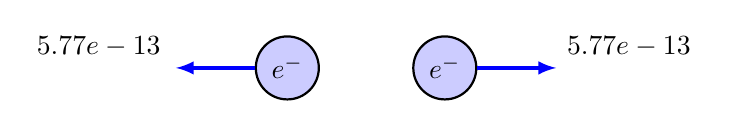
\begin{tikzpicture}[
			scale=1.0, 
			place/.style={circle,draw=black,fill=blue!20,thick,
			inner sep=0pt,minimum size=8mm},
			force/.style={>=latex,draw=blue,fill=blue, very thick, ->}
			]
			\node[place] (m1) at (-1,0) {$e^-$};
			\node[place] (m2) at (1,0)  {$e^-$};
			\draw[force] (m2.east) -- ++(1,0) node[above right] 
				{$\num{5.77e-13} \, \si{\newton}$};
			\draw[force] (m1.west) -- ++(-1,0) node[above left] 
				{$\num{5.77e-13} \, \si{\newton}$};
		\end{tikzpicture}
	\end{center}
	Þá stefnir krafturinn frá sitt hvorri rafeind og með jafnstórri stærð.
\end{formalexample}
\begin{formalexample}
	Hlutur með punkthleðsluna $\num{5} \, \si{\nano\coulomb}$ og
	rafeind liggur í óþekktri vegalengd frá rafeindinni. Hins vegar
	upplifir rafeindin kraftinn $\num{-3} \si{\micro\newton}$.
	\begin{center}
		\begin{tikzpicture}[
			scale=1.0, 
			place/.style={circle,draw=black,fill=blue!20,thick,
			inner sep=0pt,minimum size=9mm},
			force/.style={>=latex,draw=blue,fill=blue, very thick, ->}
			]
			\node[place] (m1) at (-1.5,0) {$\num{5} \, \si{\nano\coulomb}$};
			\node[place, minimum size=7mm] (m2) at (1.5,0)  {$e^-$};
			\draw[force] (m1.east) -- ++(0.6,0) node[above] 
				{$\num{3} \si{\micro\newton}$};
			\draw[force] (m2.west) -- ++(-0.6,0) node[above] 
				{$\num{3} \si{\micro\newton}$};
		\end{tikzpicture}
	\end{center}
	Finndu óþekktu vegalengdina á milli hleðslanna.
	\\[4 ex]
	Hægt er að umskrifa lögmál Coulombs sem
	\begin{align*}
		\uforce_\text{raf}
		&=
		\uconstk \frac{\uchargeq \uchargeQ}{\ulengthr^2} && \Leftrightarrow \\
		\ulengthr^2
		&=
		\uconstk \frac{\uchargeq \uchargeQ}{\uforce_\text{raf}} 
		&& \Leftrightarrow \\
		\ulengthr
		&=
		\pm \sqrt{ \uconstk \frac{\uchargeq \uchargeQ}{\uforce_\text{raf}} }
		\\
	\end{align*}
	neikvæða formerkið við rótina hefur ekki þýðingu sem lengd og því er
	það ekki notað. Þetta gefur við innsetningu
	\begin{align*}
		\ulengthr
		&=
		\sqrt{ 
			\ucoulombconstantenmc 
			\frac{ (\num{5e-9} \, \si{\coulomb}) 
				\times (\num{-1.602e-19} \, \si{\coulomb})
				}{\num{-3e-6} \si{\newton}} 
			}
		\\
		&=
		\sqrt{ 
			\num{2.3998e-12} \si{\metre\squared}
			} \\
		&=
		\num{1.55e-6} \si{\metre}
	\end{align*}
	sem þýðir að bilið á milli hleðslunnar og rafeindarinnar er
	$\num{1.55} \si{\micro\metre}$.
\end{formalexample}

\section{Superposition hleðsla}
\todo{Finna íslenskt orð fyrir superposition}% Charge
Hægt er að leggja saman kraftinn á hleðslur, þá geta margar hleðslu verkað á
eina hleðslu. Sem dæmi er hægt að skoða kraftinn sem verkar á eina hleðslu
þegar tvær hleðslur eru lagðar sitthvorum megin við hana.
\begin{center}
	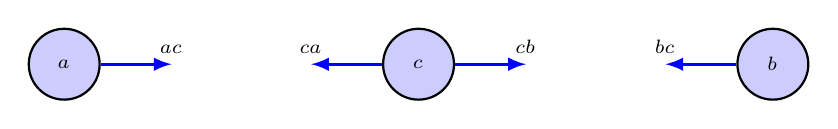
\begin{tikzpicture}[
		scale=3.0, 
		place/.style={circle,draw=black,fill=blue!20,thick,
		inner sep=0pt,minimum size=9mm},
		force/.style={>=latex,draw=blue,fill=blue, very thick, ->}
		]
		\node[place, minimum size=9mm] (m1) at (-1.5,0) {$\uforce_a$};
		\node[place, minimum size=9mm] (m2) at (1.5,0)  {$\uforce_b$};
		\node[place, minimum size=9mm] (m3) at (0,0)  {$\uforce_c$};
		\draw[force] (m1.east) -- ++(0.3,0) node[above] 
			{$\uforce_{ac}$};
		\draw[force] (m3.west) -- ++(-0.3,0) node[above] 
			{$\uforce_{ca}$};
		\draw[force] (m3.east) -- ++(0.3,0) node[above] 
			{$\uforce_{cb}$};
		\draw[force] (m2.west) -- ++(-0.3,0) node[above] 
			{$\uforce_{bc}$};
	\end{tikzpicture}
\end{center}
þá er samanlagður kraftur sem verkar á miðju hleðsluna er þá
\begin{align*}
	\uforce_\text{heild, c} &= \uforce_{ca} + \uforce_{cb}
\end{align*}
hins vegar ef það er skoðað nánar, þá heildarkrafturinn sem verkar á
allt kerfið núll. Sem virkar dálítið sérstakt nema hvað báðar hleðslurnar
verka með jafnstórum og gagnstæðum kröftum. Þá leiðir af sér að
þriðja lögmál Newtons myndar heildkraftinn núll ef enginn
utanaðkomandi kraftur verkar á kerfið þrátt fyrir innri gagnkrafta.
\begin{formalexample}
	Þrjár hleðslur liggja á beinni línu, hver er krafturinn sem verkar
	á hleðsluna C af völdum A og B?
	\begin{center}
		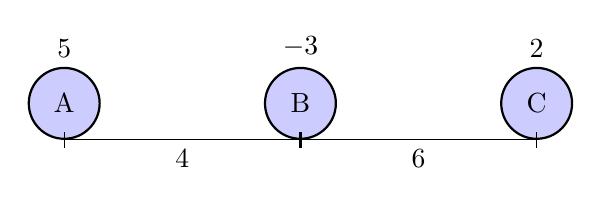
\begin{tikzpicture}[
			scale=2.0, 
			place/.style={circle,draw=black,fill=blue!20,thick,
			inner sep=0pt,minimum size=9mm},
			force/.style={>=latex,draw=blue,fill=blue, very thick, ->}
			]
			\node[place, minimum size=9mm] (m1) at (-1.5,0) {A};
			\node[place, minimum size=9mm] (m2) at (0,0)    {B};
			\node[place, minimum size=9mm] (m3) at (1.5,0)  {C};
			\draw[] (m1.north) node[above] 
				{$\SI{5}{\nano\coulomb}$};
			\draw[] (m2.north) node[above] 
				{$\SI{-3}{\nano\coulomb}$};
			\draw[] (m3.north) node[above] 
				{$\SI{2}{\nano\coulomb}$};
			\draw[|-|] (m1.south) -- (m2.south) node[pos=0.5, below] 
				{$\SI{4}{\micro\meter}$};
			\draw[|-|] (m2.south) -- (m3.south) node[pos=0.5, below] 
				{$\SI{6}{\micro\meter}$};
		\end{tikzpicture}
	\end{center}
	.
	\\[4 ex]
	Þar sem við erum með bæði jákvæðar og neikvæðar hleðslur er nauðsynlegt
	að huga að stefnu rafkraftana sem verka á hleðslu C. Við veljum að jákvæð
	kraftstefna er til hægri að vana. Fyrst er krafturinn
	á mill A og C fráhrindikraftur og samanlagt er vegalengdin á milli A og C
	$\SI{10}{\micro\meter}$. Hleðslurnar ýta hvor annari í burtu með kraftinum
	\begin{align*}
		\uforce_{ca} &=
			\uconstk \frac{\uchargeq_A \uchargeq_C}{\ulengthr_{AC}^2} \\
			&= \ucoulombconstantenmc
				\frac{
					(\SI{5e-9}{\coulomb}) 
					\times (\SI{2e-9}{\coulomb})
					}{\left( \SI{10e-6}{\meter} \right)^2} \\
			&= \SI{898}{\N}
	\end{align*}
	á svipaðan máta er hægt að finna kraftinn á milli B og C, nema hvað það
	er aðdráttarkraftur
	\begin{align*}
		\uforce_{ca} &=
			\uconstk \frac{\uchargeq_B \uchargeq_C}{\ulengthr_{BC}^2} \\
			&= \ucoulombconstantenmc
				\frac{
					(\SI{-3e-9}{\coulomb}) 
					\times (\SI{2e-9}{\coulomb})
					}{\left( \SI{6e-6}{\meter} \right)^2} \\
			&= \SI{-1498}{\N}
	\end{align*}
	þá er heildarkrafturinn á hleðslu C gefinn við 
	\begin{align*}
		\uforce_\text{heild, C} &= \SI{898}{\N} - \SI{1498}{\N} \\
			&= \SI{-600}{\N}
	\end{align*}
	þeas. hleðsla C er dregin í átt að bæði A og B vegna aðdráttarkrafts
	hleðslu B.
\end{formalexample}

\section{Eiginleikar hleðslu}
% Charge
Hleðsla er eiginleiki efnis sem er svipaður og massi, hleðsla er s.s. stærð sem
gefur mælanlegan kraft sem er ekki öðrum stærðum. Tveir helstu kraftarnir sem
koma frá eiginleikum efnis er einmitt rafkraftar og þyngdarkraftar. Hins vegar
eru fleiri kraftar sem efni getur myndað, þar af veikir og sterkir kjarnakraftar.
Hins vegar verða þeir ekki teknir fyrir hér.

\section{Rafsvið}
% Electric fields
Krafturinn sem hleðsla verkar á aðra hleðslu er í beinu samræmi við stærð
upphafshleðslu. Þá er það kraftur á hverja hleðslu einingu sem hægt er að
verka á aðrar hleðslur með. Krafurinn sem verkar á eind með tiltekna hleðslu
$q$ frá hleðslunni $Q$ er hægt að lýsa sem
\begin{align*}
	\uforce &=
			\uconstk \frac{\uchargeq \uchargeQ}{\ulengthr^2}
\end{align*} 
þá þetta kraftur sem verkar á $q$ vegna $Q$. Þá er rafsvið sama og kraftur
á hleðslu, svipað og kraftur per massa í þyngdarsviði. Þá myndi rafsviðið
vera skilgreint sem
\begin{align} \label{equ:electric:efield}
	\uefielde = \frac{ \uforce }{ \uchargeq }
\end{align}
skoðað nánar er hefur þetta eininguna $\si{\N \per \coulomb}$. Það sem ber
að huga, er að prufuhleðslan upplifir kraftinn per hleðslu í rafsviði. Þá
er hægt að ímynda sér að allar aðrar hleðslu en prufuhleðslan mynda rafsvið
sem prufuhleðslan liggur í. Þá myndi rafsviðið sem frá hleðslunni $Q$ sem
verkar á $q$ vera gefið við
\begin{align*}
	\uefielde &= \frac{ \uforce }{ \uchargeq } \\
		&= \uconstk \frac{\uchargeq \uchargeQ}{\uchargeq \ulengthr^2} \\
		&= \uconstk \frac{\uchargeQ}{\ulengthr^2}
\end{align*}
sem sagt rafsviðið sem $q$ upplifir er óháð eigin hleðslu. Þá er stefna
rafsviðs líka mikilvæg, líkt og með krafta þá getum við gefið rafsviði
stefnu. Nánar tiltekið þá getum við ímyndað okkur að jákvæðar hleðslur
hafi rafsvið sem flæðir útfrá hleðslunni, hið gagnstæða myndi vera neikvæð
hleðsla sem tekur á móti rafsviði sem flæðir í átt að neikvæðu hleðslunni.
Þá þarf að skoða hvernig kraftur hagar sér í rafsviði, krafturinn sem
hleðsla myndi upplifa er hægt að umskrifa með hjálp (\ref{equ:electric:efield})
til að vera
\begin{align}
	\uforce &= \uchargeq \uefielde
\end{align}
þá er stefna kraftins háð formerki $\uefielde$ og $\uchargeq$.
\begin{formalexample}
	Eind með hleðsluna $\SI{-5}{\micro\coulomb}$ liggur láréttu
	einsleitu rafsviði með styrkinn $\SI{10}{\N\per\coulomb}$.
	Finndu kraftinn sem hleðslan upplifir í rafsviðinu.
	\begin{center}
		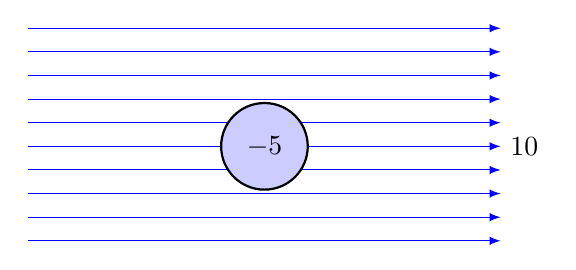
\begin{tikzpicture}[
			scale=3.0, 
			place/.style={circle,draw=black,fill=blue!20,thick,
			inner sep=0pt,minimum size=9mm},
			efield/.style={>=latex,draw=blue,fill=blue!50, thin, ->}
			]
			\foreach \x in {0.1, 0.2, ..., 1.0}
				\draw[efield] (0,\x) -- (2, \x);
			\node[place, minimum size=11mm] (m1) at (1,0.5) 
				{$\SI{-5}{\micro\coulomb}$};
			\draw (2, 0.5) node[right] {$\SI{10}{\N\per\coulomb}$};
		\end{tikzpicture}
	\end{center}
	\vspace{4 ex}
	Þá er mikilvægt að hafa stefnur vel skilgreindar, hérna stefnir
	rafsviðið til hægri og því er valin sem jákvæð stefna. Þegar við
	skoðum stærð kraftsins
	\begin{align*}
		\uforce &= \uefielde \uchargeq \\
			&= \SI{10}{\N\per\coulomb} \times \SI{-5e-6}{\coulomb} \\
			&= \SI{-5e-5}{\N} \\
			&= \SI{-500}{\mN}
	\end{align*}
	sem þýðir að krafturinn verkar gagnstætt stefnu rafsviðsins, myndrænt
	myndi krafturinn vera
	\begin{center}
		\begin{tikzpicture}[
			scale=2.0, 
			place/.style={circle,draw=black,fill=blue!20,thick,
			inner sep=0pt,minimum size=9mm},
			efield/.style={>=latex,draw=blue,fill=blue!50, thin, ->},
			force/.style={>=latex,draw=blue,fill=blue, very thick, ->}
			]
			\foreach \x in {0.1, 0.2, ..., 1.0}
				\draw[efield] (0,\x) -- (2, \x);
			\node[place, minimum size=11mm] (m1) at (1,0.5) 
				{$\SI{-5}{\micro\coulomb}$};
			\draw (2, 0.5) node[right] {$\SI{10}{\N\per\coulomb}$};
			\draw[force] (m1.west) -- ++(-0.5,0) node[above] {$\SI{-50}{\mN}$};
		\end{tikzpicture}
	\end{center}
\end{formalexample}
rafsviðið sem myndast á milli tveggja hleðsla er venjulega
ekki einsleitt eins og í fyrra dæmi. Þá er rafsviðið sem myndast
á milli tveggja hleðsla gefið \todo{make pretty lines, make tikz
plot the lines} sem
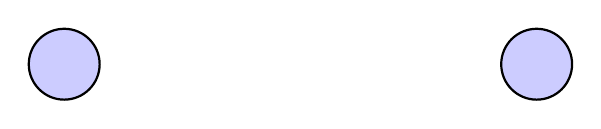
\begin{tikzpicture}[
	scale=3.0, 
	place/.style={circle,draw=black,fill=blue!20,thick,
	inner sep=0pt,minimum size=9mm},
	force/.style={>=latex,draw=blue,fill=blue, very thick, ->},
	]
	\node[place, minimum size=9mm] (m1) at (-1.0,0) {};
	\node[place, minimum size=9mm] (m2) at (1.0,0) {};
\end{tikzpicture}
eftir því hvar rafsviðið á milli hleðslanna er skoðað er það stundum
þéttara en annars. Þéttleikinn á rafsviðinu er í beinu samræmi við
línuþéttleikann á myndinni, því minna bil á milli línanna því stærri
rafsviðsstyrkurinn. Nánar tiltekið, hægt er að lesa myndina á sama
máta og hæðarlínur á kortum, því þéttari sem hæðarlínurnar eru því
meiri breyting er í hæðinni (upp eða niður).
\begin{formalexample}
	Eind með hleðsluna $\SI{5}{\micro\coulomb}$ liggur á beinni línu
	$\SI{2}{\micro\m}$ frá prufhleðslu. Finndu styrk rafsviðsins
	og kraftinn sem prufuhleðslan upplifir ef hún er rafeind.
	\vspace{4 ex}
	
	\noindent Styrkur rafsviðsins sem prufuhleðslan upplifir er einungis háð
	hleðslu eindarinnar, þeas.
	\begin{align*}
	\uefielde
		&= \uconstk \frac{\uchargeQ}{\ulengthr^2} \\
		&= \ucoulombconstantenmc \times
			\frac{\SI{5e-6}{\coulomb}
				}{
				\left( \SI{2e-6}{\m} \right)^2
				} \\
		&= \SI{11.235e15}{\N\per\coulomb} \\
		&= \SI{11.235}{\peta\N\per\coulomb}
	\end{align*}
	sem er ótrúlegur kraftur á hvert Coulomb, ef við skoðum
	kraftinn sem rafeind myndi upplifa í þessu rafsviði þá fæst
	\begin{align*}
		\uforce &= \uefielde \uchargeq \\
			&= \SI{11.235e15}{\N\per\coulomb} \times \SI{-1.602e-19}{\coulomb} \\
			&= \SI{-17.998e-3}{\N} \\
			&= \SI{-18}{\mN}
	\end{align*}
	þá er krafturinn talsvert minni, oft eru rafsvið með gríðarlega styrk en
	stærð kraftsins sem verkar á prufuhleðsluna er í beinu samræmi við eigin
	hleðslu. Þá tvær rafeind myndu upplifa tvöfalda hleðslu.
\end{formalexample}
 

\section{Þyngdar- og rafsvið}
% Similarities between gravity and electric force
Þegar við vinnum hluti sem verða fyrir krafti í fjarlægð, þá er hægt að koma
með samlíkingu á milli áhrifa. Það er svipað mynstur sem bæði rafkraftar
og þyngdarkraftar fylgja. Báðir kraftar hafa öfugt hlutfall við vegalengdina
á milli einda (hleðslur eða massar), þá er almment átt við
\begin{align*}
	F \propto \frac{1}{r^2}
\end{align*}
sem er eins hlutfall fyrir báða krafta. Hins vegar verður lesandi að fara
varlega hvaða ályktanir er hægt að draga af slíku samræmi. Það geti verið
ábending um að það bæði þyngdar- og rafkraftar eru tvö form af sama kraftinum,
nema að þyngdakraftur hefur ekki getað samræmst öðrum kröftum sem heilstætt
líkan fyrir alla krafta. Hægt er að samræma þrjá af fjórum þekktum kröftum
sem eru taldnir stýra alheiminum, nema þyngdarkraftinum, sér í lagi vegna
þess hversu lítill hann er miðað við hina þrjá kraftana.

Þetta er mjög gott dæmi um að fylgni stærða er ekki nauðsynlega vegna
gagnkvæmna afleiðinga, þeas. sem stendur þá lítur út fyrir að
þyngdarkrafturinn er sér á báti.

\section{Fasti couloumbs}
% How it is derived

